\section{Introduction}
\label{sec:intro}
The world wide web is by far the largest source of information today.
Much of that information contains structured data such as tables and lists
which are very valuable for knowledge discovery and data mining. 
This structured data is valuable not only because of the relational
values it contains, but also because it is relatively easier to unlock
information from data with some regular patterns than free text which
makes up most of the web content. However, when encoded in HTML, 
structured data becomes {\em semi-structured}. 
And because HTML is designed for rendering in a browser, different
HTML code segments can give the same visual effect at least to
the human eye. As a result, 
HTML coding is much less stringent than XML, and
inconsistencies and errors are abundant in HTML documents. 
All these pose significant challenges in the extraction of structured 
data from the web \cite{Weninger10:UnexpectedList}.

In this demo, we focus on list data in web pages. In particular, we are 
interested in extracting from a kind of web pages which present
a list of $k$ instances of a topic or a concept. Examples of such topic include 
``20 Most Influential Scientists Alive Today'', 
``Ten Hollywood Classics You Shouldn't Miss'', 
and ``50 Tallest Persons in the World''. 
We call these pages ``top-$k$'' pages.
Figure \ref{fig:topscientists}
shows one such ``top-$k$'' page \cite{InfluentialScientists}.
Figure \ref{fig:topscientists}.(a) is a snapshot of the page 
and Figure \ref{fig:topscientists}.(b-d) are some of its segments.
The title (Figure \ref{fig:topscientists}.(b)) of a ``top-$k$'' page 
usually contains a number $k$ indicating the list size (20),
as well as the head word/phrase (e.g., scientist) which best describes 
the entities in the list. Figure \ref{fig:topscientists}.(c) shows one 
instance (element) in the list, which not only contains the instance name 
(Timothy J. Berners-Lee), but also optionally additional information like 
a picture, a textual description and a link to a relevant wikipedia page. 
The additional information can be treated as the attributes of the instance. 
A ``top-$k$'' page can also contain unwanted lists
such as Figure \ref{fig:topscientists}.(d) which
should be filtered out.

\begin{figure*}[th]
        \centering
        \epsfig{file=./pic/page5_detail.eps,width=1.8\columnwidth}
        \caption{Snapshot of a typical  ``top-k'' page
	\cite{InfluentialScientists} and its page segments}
        \label{fig:topscientists}
\end{figure*}
Our system is designed to extract ``top-$k$'' lists from web pages.
Basically, it performs three tasks:
1) Recognize a ``top-$k$'' page;
2) Extract the ``top-$k$'' list;
3) Understand and process list content. 

The input of the system is any HTML web page 
and the output is the extracted ``top-$k$'' list of the page, if any.
Table \ref{tab:sampleoutput} shows the sample output from the page shown in
Figure \ref{fig:topscientists}.
\footnote{The actual output is stored in XML format and includes additional information.}

\begin{table*}
\centering
\begin{tabular}{|l|l|l|l|l|} \hline
{\bf Index} & {\bf Name} & {\bf Image} & {\bf Description} & {\bf Wiki. Link} \\ \hline
1 & {\em Timothy J. Berners-Lee} & tim-berners-lee\_1366736c.jpg & who invented the World Wide Web... & [link]\\ 
2 & {\em Noam Chomsky} & noam\_chomsky.jpg & who, though a linguist and philosopher... & [link]\\ 
3 & {\em Richard Dawkins} & richard\_dawkins.jpg &  whose use of evolutionary biology has shaped... & [link] \\ 
...& ... & ... & ... & ... \\
20 & {\em Edward Witten} & edward\_witten.jpg & whose work on the mathematical 
underpinnings... & [link] \\
\hline
\end{tabular}
\caption{Sample extraction output of ``20 Most Influential Scientists Alive Today'' \cite{InfluentialScientists}}
\label{tab:sampleoutput}
\end{table*}

There were many previous attempts to extract lists or tables from the web.
None of them targets the ``top-$k$'' list extraction that is studied in
this work. In fact, most of the methods are based on either very specific
list-related tags 
%\cite{googlesets,webtables08} 
\cite{webtables08} 
such as {\tt <ul>}, {\tt <li>} and {\tt <table>} 
or the similarity between DOM trees 
\cite{LiuGZ03:MDR,MiaoTHSM09:TagPathClustering} and ignore
the visual aspect of HTML documents. These approaches are likely to be
brittle because of the dynamic and inconsistent nature of web
pages. More recently, several groups
have attempted to utilize visual information in HTML in 
information extraction. Most notably, Ventex 
\cite{GatterbauerBHKP2007:Towards} and HyLiEn \cite{FumarolaWBMH11:List} 
were designed to correlate the rendered visual model or features
with the corresponding DOM structure and achieved remarkable improvements
in performance. However, these techniques indiscriminatingly extract {\em all}
elements of {\em all} lists or tables from a web page, therefore the objective
is different from that of this work which is to extract {\em one} specific
list from a page while purging all other lists (e.g. (d) in
Figure \ref{fig:topscientists}) as noise. The latter poses
different challenges such as distinguishing ambiguous list boundaries
and identifying unwanted lists. 

We target ``top-$k$'' list data for information extraction 
for the following reasons.
%Besides, compared with normal web tables and lists, ``top-$k$'' lists are more important for the following reasons:
First, there are {\em large} amount of ``top-$k$'' lists around on the web. 
We estimate that the total number in Bing's corpus is around 2.24 million 
(1.4\textperthousand~ of total number of pages), 
and our system can effectively extract up to 75.5\% of them. 
The scale of this data is larger than any manually or automatically 
extracted lists in the past.

Second, list data is generally {\em cleaner} than other forms of web data.
Free text contains a lot of variation and ambiguity and is known to be hard
to understand and extract. General tables, even though structured, 
can have many different forms (such as row span and column span) and styles, 
and many of them are not meaningful if we don't
know the schema of the table or the meaning of the headers 
\cite{WangWWZ12:Tables}.
Lists, on the other hand, have relatively simpler structures and are easier to
identify. What's more, ``top-$k$'' lists, with their unique semantics, are even
cleaner than ordinary lists.
%on the web. General tables and lists extracted from Internet 
%contain a lot of noises such as advertisements and comments,
%which are often useless for further analysis; while our system can filter those unwanted data
%and extract ``top-$k$'' list with up to 90\% precision(see Section 
%\ref{sec:eval}).

Third, ``top-$k$'' lists are relatively {\em easier} to understand. 
``top-$k$'' list pages share a common style: 
the title contains a number and 
the topic or concept of the list. 
Each list item can be considered as an instance of the page title. 
The number of items should be equal to the number mentioned in the title.
Besides the name of the instance, each list item 
may contain additional attributes of the instance.

Finally, ``top-$k$'' lists have {\em interesting} semantics. 
The fact that the list items
are called ``top XXX'' means that these items are more important, popular or 
meaningful than an arbitrary list. What's more, people are always fascinated
about rankings. Information of this sort is likely to find a 
large audience.  

%Since the input of our system are independent,
%we can easily deploy it onto some Map/Reduce system,
%in order to process massive web pages.
We deployed our prototype system on a distributed computing platform
and performed extraction on up to 1/10 of a high frequency web snapshot
crawled by Bing. Our preliminary results showed that the system achieved
90.4\% precision and 57.7\% recall. That amounts to the correct
extraction of 129,169 lists from a total of 160 million randomly selected 
web pages. 

The work described in this paper is an important step in our bigger effort of 
automatic constructing a universal knowledge base 
that includes large number of known concepts and their instances. 
To that end, we have already built one of the largest open-domain taxonomy 
called Probase \cite{WuLWZ12:Probase,WangLWZ12:Topic,WangWWZ12:Tables,Song11:Conceptualize} 
which consists of 2.7 million concepts and many more instances. 
The ``top-$k$'' lists we extracted from the web can be an important source 
for enriching Probase's instance space.
Also, our system enables the construction of
an effective fact answer engine \cite{YinTL11:Facto}. 
With such an engine, we can answer queries such as
``Who are the 10 tallest persons in the world'', or ``What are 50 best-selling
books in 2010'' directly, instead of referring the users to a set of ranked
pages like all search engines do today. 

Next we will briefly discuss the framework of our system 
(Section \ref{sec:algo}) and the preliminary evaluation results 
(Section \ref{sec:eval}), and present a plan for demonstration (Section
\ref{sec:demo}).  
